% ------------------------------------------------------------------------------
% TYPO3 CMS 7.6 - What's New - Chapter "In-Depth Changes" (English Version)
%
% @author	Patrick Lobacher <patrick@lobacher.de> and Michael Schams <schams.net>
% @license	Creative Commons BY-NC-SA 3.0
% @link		http://typo3.org/download/release-notes/whats-new/
% @language	English
% ------------------------------------------------------------------------------
% LTXE-CHAPTER-UID:		7229f1b9-b481e9bc-09c46183-a86b6a7e
% LTXE-CHAPTER-NAME:	In-Depth Changes
% ------------------------------------------------------------------------------

\section{In-Depth Changes}
\begin{frame}[fragile]
	\frametitle{In-Depth Changes}

	\begin{center}\huge{Capitolo 3:}\end{center}
	\begin{center}\huge{\color{typo3darkgrey}\textbf{Modifiche rilevanti}}\end{center}

\end{frame}

% ------------------------------------------------------------------------------
% LTXE-SLIDE-START
% LTXE-SLIDE-UID:	a9c37cdf-b2b0b24d-31138e4f-5396662f
% LTXE-SLIDE-ORIGIN:	159a2d7f-b679989c-30cf1736-6693f827 English
% LTXE-SLIDE-TITLE:		Bootstrap for Install Tool (1)
% ------------------------------------------------------------------------------

\begin{frame}[fragile]
	\frametitle{In-Depth Changes}
	\framesubtitle{Install Tool con Bootstrap (1)}

	\begin{itemize}

		\item L'Install Tool è basato su Bootstrap - per la parte di installazione:

			\begin{figure}
				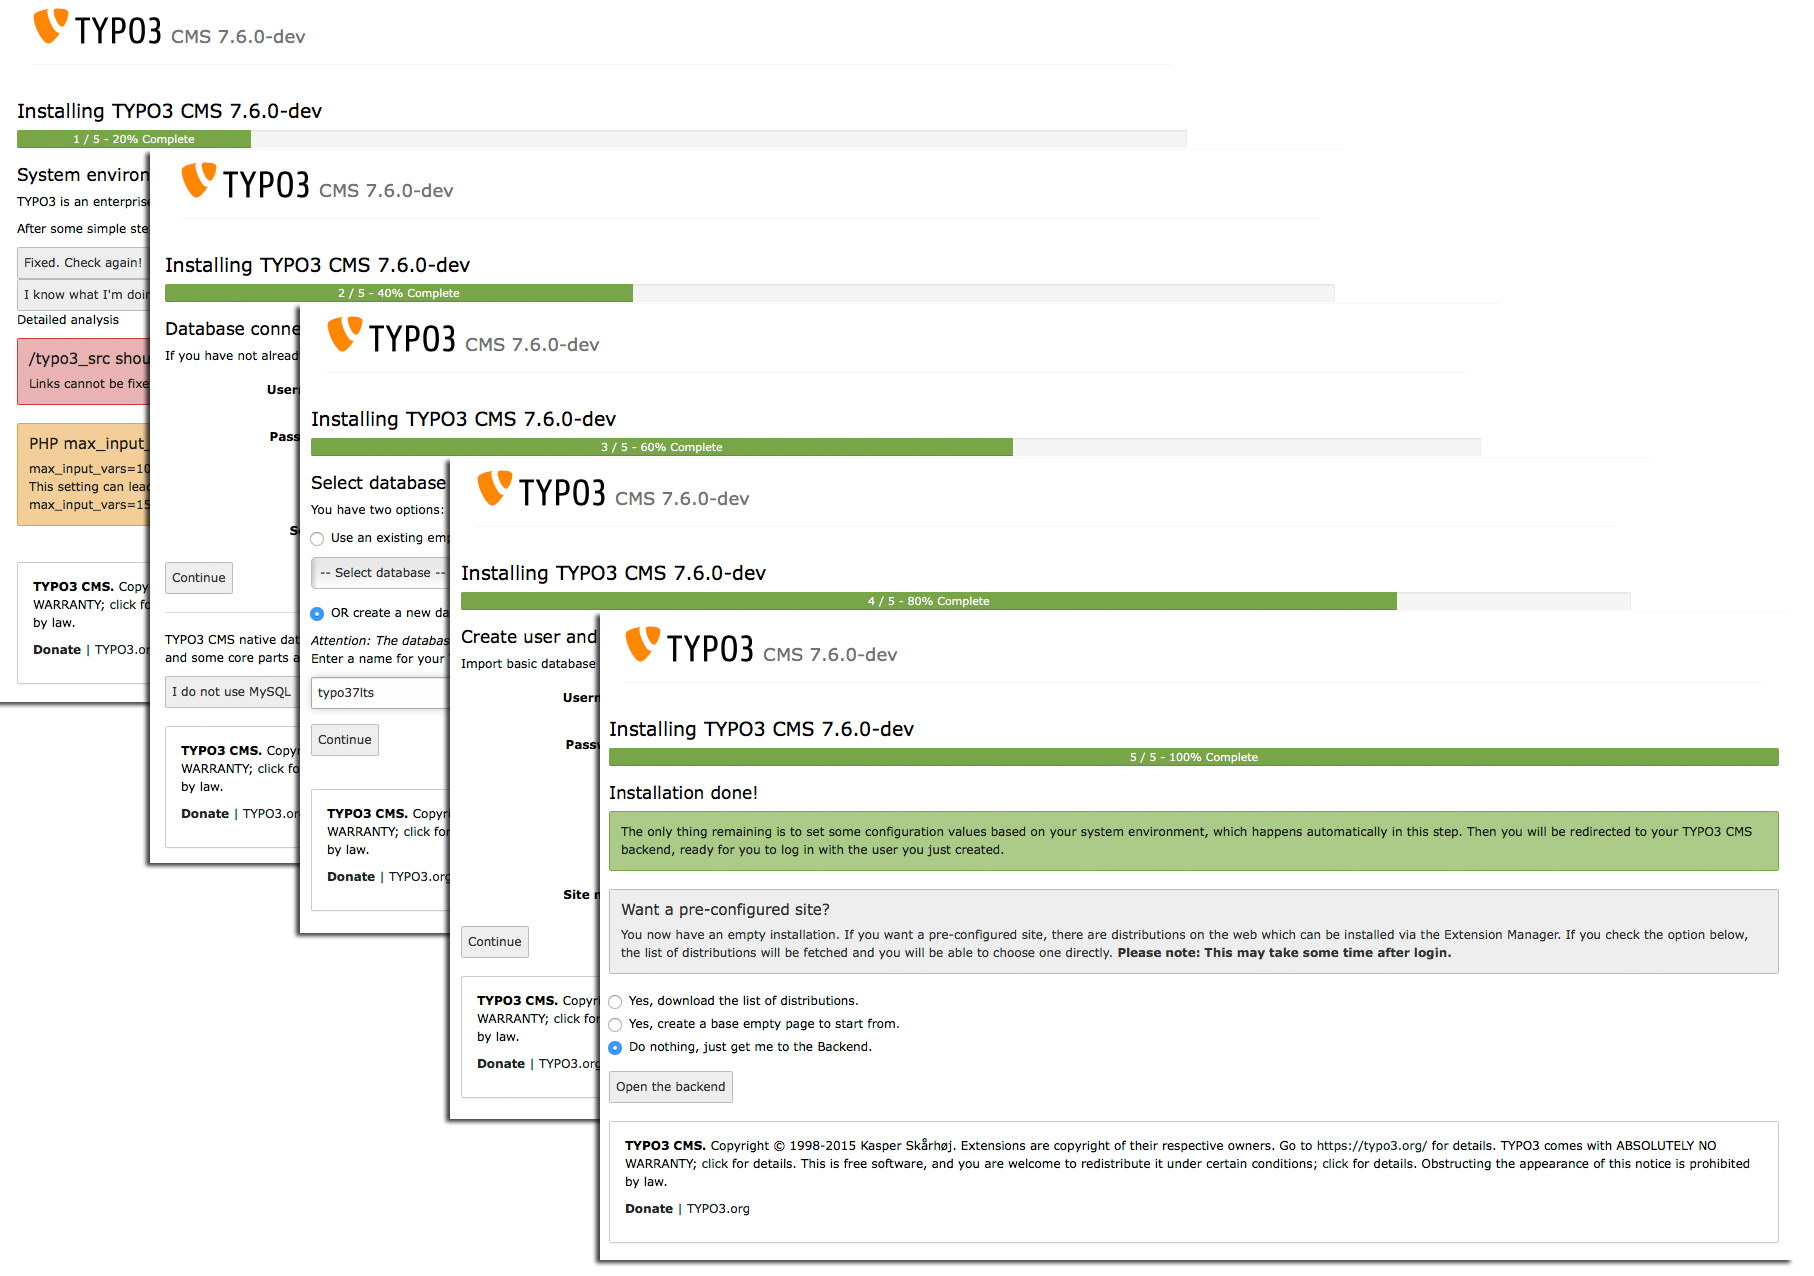
\includegraphics[width=0.7\linewidth]{InDepthChanges/InstallToolBootstrap01.jpg}
			\end{figure}

	\end{itemize}

\end{frame}

% ------------------------------------------------------------------------------
% LTXE-SLIDE-START
% LTXE-SLIDE-UID:		96f80c84-93c037e4-e4dcb6aa-832e6f72
% LTXE-SLIDE-ORIGIN:	66a71f73-91b6c90e-e548a037-e2d47f94 English
% LTXE-SLIDE-TITLE:		Bootstrap for Install Tool (2)
% ------------------------------------------------------------------------------

\begin{frame}[fragile]
	\frametitle{In-Depth Changes}
	\framesubtitle{Install Tool con Bootstrap (2)}

	\begin{itemize}

		\item L'Install Tool è basato su Bootstrap - per la parte di configutazione:

			\begin{figure}
				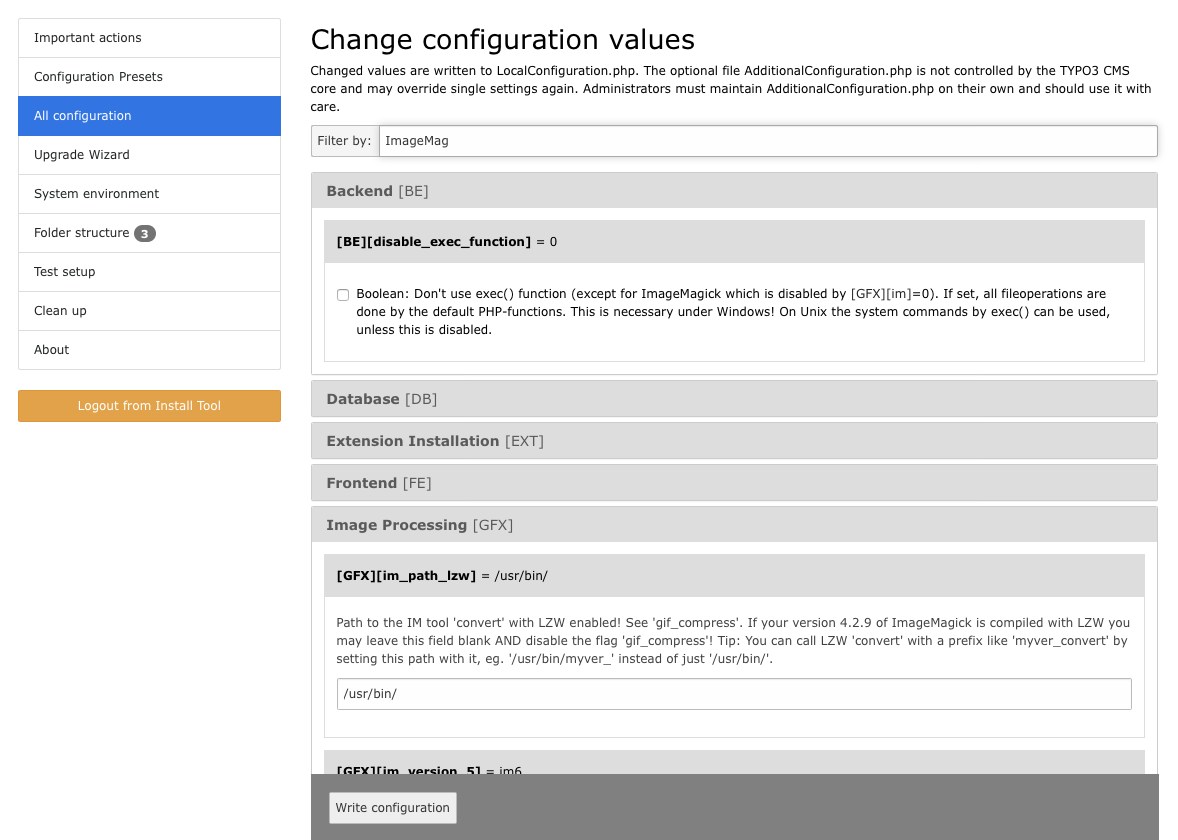
\includegraphics[width=0.7\linewidth]{InDepthChanges/InstallToolBootstrap02.png}
			\end{figure}

	\end{itemize}

\end{frame}

% ------------------------------------------------------------------------------
% LTXE-SLIDE-START
% LTXE-SLIDE-UID:		4c857267-4ad5e116-79ea2288-d30b85e9
% LTXE-SLIDE-ORIGIN:	f901074a-4080140f-dd93e505-1e8c2178 English
% LTXE-SLIDE-ORIGIN:	d5acb2d2-159a2d7f-6693f827-30cf1736 German
% LTXE-SLIDE-TITLE:		Form protection API for frontend usage
% LTXE-SLIDE-REFERENCE:	Feature-56633-FormProtectionAPIForFrontEndUsage.rst
% ------------------------------------------------------------------------------

\begin{frame}[fragile]
	\frametitle{Modifiche rilevanti}
	\framesubtitle{Protezione CSRF per i Plugin di Frontend}

	% decrease font size for code listing
	\lstset{basicstyle=\tiny\ttfamily}

	\begin{itemize}

		\item Una nuova classe permette l'uso delle API FormProtection nel frontend

		\item Queste implementano un protezione CSRF (Cross-Site Request Forgery)

			\begin{lstlisting}
				$formToken = \TYPO3\CMS\Core\FormProtection\FormProtectionFactory::get()->getFormProtection()->generateToken('news', 'edit', $uid);
				if (
				  $dataHasBeenSubmitted
				  && \TYPO3\CMS\Core\FormProtection\FormProtectionFactory::get()->validateToken(
				    \TYPO3\CMS\Core\Utility\GeneralUtility::_POST('formToken'), 'User setup', 'edit')) {
				  // processes the data
				}
				else {
				  // invalid token!
				}
			\end{lstlisting}

	\end{itemize}

\end{frame}

% ------------------------------------------------------------------------------
% LTXE-SLIDE-START
% LTXE-SLIDE-UID:		781f9882-1ef5a7b1-6cd7115d-c3712e0e
% LTXE-SLIDE-ORIGIN:	0198b067-68da7843-6a6d3f6d-94cee9b7 English
% LTXE-SLIDE-ORIGIN:	388c7243-b679989c-e2b30dbb-78f1aea4 German
% LTXE-SLIDE-TITLE:		Added LinkBrowser APIs (1)
% LTXE-SLIDE-REFERENCE:	Feature-66369-AddedLinkBrowserAPIs.rst
% ------------------------------------------------------------------------------

\begin{frame}[fragile]
	\frametitle{Modifiche rilevanti}
	\framesubtitle{Tab per LinkBrowser (1)}

	% decrease font size for code listing
	\lstset{basicstyle=\tiny\ttfamily}

	\begin{itemize}

		\item Questa nuova funzionalità permette di estendere il LinkBrowser con nuovi tab

		\item Ogni tab è gestito fa un cosiddtto "LinkHandler", il quale deve implementare le
			seguenti Interfacce:\newline
			\small
				\texttt{\textbackslash TYPO3\textbackslash CMS\textbackslash Recordlist\textbackslash LinkHandler\textbackslash LinkHandlerInterface}
			\normalsize

		\item I LinkHandler sono registrati in PageTSconfig come segue:

			\begin{lstlisting}
				file {
				  handler = TYPO3\\CMS\\Recordlist\\LinkHandler\\FileLinkHandler
				  label = LLL:EXT:lang/locallang_browse_links.xlf:file
				  displayAfter = page
				  scanAfter = page
				  configuration {
				    customConfig = passed to the handler
				  }
				}
			\end{lstlisting}

	\end{itemize}

\end{frame}

% ------------------------------------------------------------------------------
% LTXE-SLIDE-START
% LTXE-SLIDE-UID:		63fb6d06-e23b7074-5e83dec7-4266e8ce
% LTXE-SLIDE-ORIGIN:	7ff322bc-2ace574c-34ddebb5-559fd90c English
% LTXE-SLIDE-ORIGIN:	dfd89b4b-7b4b816c-e5904ba8-2527339b German
% LTXE-SLIDE-TITLE:		Added LinkBrowser APIs (2)
% LTXE-SLIDE-REFERENCE:	Feature-66369-AddedLinkBrowserAPIs.rst
% ------------------------------------------------------------------------------

\begin{frame}[fragile]
	\frametitle{Modifiche rilevanti}
	\framesubtitle{Tab per LinkBrowser (2)}

	% decrease font size for code listing
	\lstset{basicstyle=\tiny\ttfamily}

	\begin{itemize}

		\item Le opzioni \texttt{displayBefore} e \texttt{displayAfter} definiscono la posizione dei tab

		\item Le opzioni \texttt{scanBefore} e \texttt{scanAfter} definiscono l'ordine in cui gli handler sono
			elaborati quando vengono verificati i link esistenti

			\begin{lstlisting}
				$GLOBALS['TYPO3_CONF_VARS']['SC_OPTIONS']['LinkBrowser']['hooks'][1444048118] = [
				  'handler' => \Vendor\Ext\MyClass::class,
				  'before' => [], // optional
				  'after' => [] // optional
				];
			\end{lstlisting}

	\end{itemize}

\end{frame}

% ------------------------------------------------------------------------------
% LTXE-SLIDE-START
% LTXE-SLIDE-UID:		48403d53-bc6ce131-7323dcbc-effb3dde
% LTXE-SLIDE-ORIGIN:	1ef90646-4f4342dd-3bf0112b-95acba1b English
% LTXE-SLIDE-ORIGIN:	687f24a3-032124a3-7ac41f15-26329962 German
% LTXE-SLIDE-TITLE:		Module Template API (1)
% LTXE-SLIDE-REFERENCE:	Feature-69814-ModuleTemplateAPI.rst
% ------------------------------------------------------------------------------

\begin{frame}[fragile]
	\frametitle{Modifiche rilevanti}
	\framesubtitle{API del modulo Template (1)}

	% decrease font size for code listing
	\lstset{basicstyle=\tiny\ttfamily}

	\begin{itemize}

		\item Le nuove API del modulo Template API hanno lo scopo di normalizzare l'implementazione di DocHeaders

		\item Esempio 1: aggiungere un bottone

			\begin{lstlisting}
				$openInNewWindowButton = $this->moduleTemplate->getDocHeaderComponent()->getButtonBar()
				  ->makeLinkButton()
				  ->setHref('#')
				  ->setTitle($this->getLanguageService()->sL(
				    'LLL:EXT:lang/locallang_core.xlf:labels.openInNewWindow', TRUE
				    ))
				  ->setIcon($this->iconFactory->getIcon('actions-window-open', Icon::SIZE_SMALL))
				  ->setOnClick($aOnClick);

				$this->moduleTemplate->getDocHeaderComponent()->getButtonBar()
				  ->addButton($openInNewWindowButton, ButtonBar::BUTTON_POSITION_RIGHT);
			\end{lstlisting}
	\end{itemize}

\end{frame}

% ------------------------------------------------------------------------------
% LTXE-SLIDE-START
% LTXE-SLIDE-UID:		65bf0c13-1f76355b-30768762-b78c2bdb
% LTXE-SLIDE-ORIGIN:	44c8e88e-5668ccb6-3cf424ea-c6a40ecf English
% LTXE-SLIDE-ORIGIN:	1570c8c9-2dfa48e9-058d2d04-bff5465d German
% LTXE-SLIDE-TITLE:		Module Template API (2)
% LTXE-SLIDE-REFERENCE:	Feature-69814-ModuleTemplateAPI.rst
% ------------------------------------------------------------------------------

\begin{frame}[fragile]
	\frametitle{Modifiche rilevanti}
	\framesubtitle{API del modulo Template (2)}

	% decrease font size for code listing
	\lstset{basicstyle=\tiny\ttfamily}

	\begin{itemize}
		\item Esempio 2: aggiungere un menu con delle voci

			\begin{lstlisting}
				$languageMenu = $this->moduleTemplate->getDocHeaderComponent()
				  ->getModuleMenuRegistry()->makeMenu()
				  ->setIdentifier('_langSelector')
				  ->setLabel($this->getLanguageService()->sL(
				    'LLL:EXT:lang/locallang_general.xlf:LGL.language', TRUE
				  ));

				$menuItem = $languageMenu->makeMenuItem()
				  ->setTitle($lang['title'] . $newTranslation)
				  ->setHref($href);

				if((int)$lang['uid'] === $currentLanguage) {
				  $menuItem->setActive(TRUE);
				}

				$languageMenu->addMenuItem($menuItem);
				$this->moduleTemplate->getDocHeaderComponent()->getModuleMenuRegistry()->addMenu($languageMenu);
			\end{lstlisting}
	\end{itemize}

\end{frame}


% ------------------------------------------------------------------------------
% LTXE-SLIDE-START
% LTXE-SLIDE-UID:		0f8c7a96-ddbb8396-a0b44c32-48071076
% LTXE-SLIDE-ORIGIN:	2ffbc623-117a44dc-923610ec-78a3afc2 English
% LTXE-SLIDE-ORIGIN:	df3ea848-d5406e98-edbd6684-485ff477 German
% LTXE-SLIDE-TITLE:		PSR-7-based Routing for Backend AJAX Requests
% LTXE-SLIDE-REFERENCE:	Feature-69916-PSR-7-basedRoutingForBackendAJAXRequests.rst
% ------------------------------------------------------------------------------

\begin{frame}[fragile]
	\frametitle{Modifiche rilevanti}
	\framesubtitle{Routing PSR-7 per le richieste AJAX di Backend}

	% decrease font size for code listing
	\lstset{basicstyle=\tiny\ttfamily}

	\begin{itemize}

		\item Per aggiungere un route per una richiesta AJAX, il file
			\texttt{Configuration/Backend/AjaxRoutes.php}\newline
			può essere creato con il seguente contenuto:

			\begin{lstlisting}
				return [
				  // fai qualcosa
				  'unique_route_name' => [
				    'path' => '/toolcollection/some-action',
				    'target' => \Vendor\Controller\SomeController::class . '::myAction',
				  ]
				];
			\end{lstlisting}

	\end{itemize}

\end{frame}

% ------------------------------------------------------------------------------
% LTXE-SLIDE-START
% LTXE-SLIDE-UID:		b6ee33ff-d3853e52-43e7a57a-e8ebce47
% LTXE-SLIDE-ORIGIN:	b68a9d26-30e6d4a0-7bccecf2-ad1f93c6 English
% LTXE-SLIDE-ORIGIN:	cb01cca6-58e91977-d18fa0b3-cba021ab German
% LTXE-SLIDE-TITLE:		Introduced two new Hooks for OpenID (getUserRecord)
% LTXE-SLIDE-REFERENCE:	Feature-44127-HooksForOpenIdToAutomaticallyCreateUserAccounts.rst
% ------------------------------------------------------------------------------
\begin{frame}[fragile]
	\frametitle{Modifiche rilevanti}
	\framesubtitle{Hook OpenID \texttt{getUserRecord}}

	% decrease font size for code listing
	\lstset{basicstyle=\tiny\ttfamily}

	Due hook sono stati aggiunti al servizio OpenID (1/2)

		\begin{itemize}

			\item Hook 1:\newline
				\smaller\smaller
					\texttt{\$GLOBALS['TYPO3\_CONF\_VARS']['SC\_OPTIONS']['openid']['getUserRecord']}
				\normalsize

				\begin{itemize}
					\item Modifica il record utente dopo che esso è stato recuperato, o:
					\item Crea un nuovo record se nessuno è stato trovato
					\item I parametri \texttt{record}, \texttt{response} e \texttt{authInfo} sono passati all'hook
				\end{itemize}

		\end{itemize}

\end{frame}

% ------------------------------------------------------------------------------
% LTXE-SLIDE-START
% LTXE-SLIDE-UID:		02f13325-1340d3f6-50d19ff1-21adb511
% LTXE-SLIDE-ORIGIN:	b9b259e4-9d35ace7-edff1014-7390d1d1 English
% LTXE-SLIDE-ORIGIN:	ea0bfed8-831666d7-1ba40bb9-7a95723a German
% LTXE-SLIDE-TITLE:		Introduced two new Hooks for OpenID (authRequest)
% LTXE-SLIDE-REFERENCE:	Feature-44127-HooksForOpenIdToAutomaticallyCreateUserAccounts.rst
% ------------------------------------------------------------------------------
\begin{frame}[fragile]
	\frametitle{Modifiche rilevanti}
	\framesubtitle{Hook OpenID \texttt{authRequest}}

	% decrease font size for code listing
	\lstset{basicstyle=\tiny\ttfamily}

	Due hook sono stati aggiunti al servizio OpenID (2/2)

		\begin{itemize}

			\item Hook 2:\newline
				\smaller\smaller
					\texttt{\$GLOBALS['TYPO3\_CONF\_VARS']['SC\_OPTIONS']['openid']['authRequest']}
				\normalsize

				\begin{itemize}
					\item Modifica la richiesta di autenticazione, prima che essa sia inviata
					\item Può essere usato per richiedere attributi aggiuntivi come un nickname dal server OpenID per esempio
					\item I parametri \texttt{authRequest} e \texttt{authInfo} sono passati all'hook
				\end{itemize}

		\end{itemize}

\end{frame}

% ------------------------------------------------------------------------------
% LTXE-SLIDE-START
% LTXE-SLIDE-UID:		7ad092d8-5474b987-7f157436-772dcf15
% LTXE-SLIDE-ORIGIN:	1626edc6-8d93ff84-f64178bf-8e7650df English
% LTXE-SLIDE-ORIGIN:	115a4459-3653bb99-1680d6ab-d8c3c69b German
% LTXE-SLIDE-TITLE:		Hook in BackendUserAuthentication::getDefaultUploadFolder (1)
% LTXE-SLIDE-REFERENCE:	Feature-68895-IntroducedHookInBackendUserAuthenticationgetDefaultUploadFolder.rst
% ------------------------------------------------------------------------------
\begin{frame}[fragile]
	\frametitle{Modifiche rilevanti}
	\framesubtitle{Hook e Signals (1)}

	% decrease font size for code listing
	\lstset{basicstyle=\tiny\ttfamily}

	\begin{itemize}

		\item Ora è possibile modificare la directory di upload restituita da
			\texttt{BackendUserAuthentication::getDefaultUploadFolder()}

		\item Registra l'hook nel file \texttt{ext\_localconf.php} come segue:

			\begin{lstlisting}
				$GLOBALS['TYPO3_CONF_VARS']['SC_OPTIONS']['t3lib/class.t3lib_userauthgroup.php']
				  ['getDefaultUploadFolder'][] =
				  \Vendor\MyExtension\Hooks\DefaultUploadFolder::class . '->getDefaultUploadFolder';
			\end{lstlisting}

	\end{itemize}

\end{frame}

% ------------------------------------------------------------------------------
% LTXE-SLIDE-START
% LTXE-SLIDE-UID:		30f0cc4e-f1148d5d-0f68f793-c3e19b57
% LTXE-SLIDE-ORIGIN:	9c150d50-ee3ba19b-120ef653-e714135c English
% LTXE-SLIDE-ORIGIN:	d1041967-32814ee3-2172e570-4a6d21bd German
% LTXE-SLIDE-TITLE:		Hook in BackendUserAuthentication::getDefaultUploadFolder (2)
% LTXE-SLIDE-REFERENCE:	Feature-68895-IntroducedHookInBackendUserAuthenticationgetDefaultUploadFolder.rst
% ------------------------------------------------------------------------------
\begin{frame}[fragile]
	\frametitle{Modifiche rilevanti}
	\framesubtitle{Hooks e Signals (2)}

	% decrease font size for code listing
	\lstset{basicstyle=\tiny\ttfamily}

	\small Esempio:\normalsize

		\begin{lstlisting}
			<?php
			namespace Vendor\MyExtension\Hooks;
			use TYPO3\CMS\Core\Authentication\BackendUserAuthentication;
			use TYPO3\CMS\Core\Resource\Folder;

			/**
			 * Class DefaultUploadFolder
			 */
			class DefaultUploadFolder {

			  /**
			   * Get default upload folder
			   * If there is a folder present with the same name as the last part of the table name use that folder.
			   * @param array $params
			   * @param BackendUserAuthentication $backendUserAuthentication
			   * @return Folder
			   */
			   public function getDefaultUploadFolder($params, BackendUserAuthentication $backendUserAuthentication) {
			    [...]
		\end{lstlisting}

\end{frame}

% ------------------------------------------------------------------------------
% LTXE-SLIDE-START
% LTXE-SLIDE-UID:		1b1838e0-9957b165-d37fb7d7-ee18a553
% LTXE-SLIDE-ORIGIN:	a4d7bec0-6c19d8b2-6a6be951-5d5aa0c0 English
% LTXE-SLIDE-ORIGIN:	2f855107-2262065c-c865f953-91b4f0ea German
% LTXE-SLIDE-TITLE:		Hook in BackendUserAuthentication::getDefaultUploadFolder (3)
% LTXE-SLIDE-REFERENCE:	Feature-68895-IntroducedHookInBackendUserAuthenticationgetDefaultUploadFolder.rst
% ------------------------------------------------------------------------------
\begin{frame}[fragile]
	\frametitle{Modifiche rilevanti}
	\framesubtitle{Hooks e Signals (3)}

	% decrease font size for code listing
	\lstset{basicstyle=\tiny\ttfamily}

	\small Esempio (continua):\normalsize

		\begin{lstlisting}
			    [...]

			    /** @var Folder $uploadFolder */
			    $uploadFolder = $params['uploadFolder'];
			    $pid = $params['pid'];
			    $table = $params['table'];
			    $field = $params['field'];

			    $matches = [];
			    if (!empty($uploadFolder) && preg_match('/_([a-z]+)$/', $table, $matches)) {
			      $folderName = $matches[1];
			      if ($uploadFolder->hasFolder($folderName)) {
			        $uploadFolder = $uploadFolder->getSubfolder($folderName);
			      }
			    }
			    return $uploadFolder;
			  }
			}
		\end{lstlisting}

\end{frame}

% ------------------------------------------------------------------------------
% LTXE-SLIDE-START
% LTXE-SLIDE-UID:		d1d86fb8-042b73a3-4a3c71fc-1bb1d016
% LTXE-SLIDE-ORIGIN:	2c656d9e-38b9be7a-d590cb6e-21eccd4d English
% LTXE-SLIDE-ORIGIN:	cd6ba83d-9f068dee-b8887ffa-4a2eff29 German
% LTXE-SLIDE-TITLE:		Diverse Änderungen
% LTXE-SLIDE-REFERENCE:	Deprecation-69822-DeprecateSelectFieldTca.rst
% ------------------------------------------------------------------------------
\begin{frame}[fragile]
	\frametitle{Modifiche rilevanti}
	\framesubtitle{Varie}

	\begin{itemize}

		\item L'uso del campo TCA di tipo \texttt{select} richiede di specificare l'opzione \texttt{renderType}

		\item I valori validi sono:

			\begin{lstlisting}
				'renderType' => 'selectMultipleSideBySide',
				'renderType' => 'selectCheckBox',
				'renderType' => 'selectSingle',
				'renderType' => 'selectSingleBox',
				'renderType' => 'selectTree',
			\end{lstlisting}

	\end{itemize}

\end{frame}

% ------------------------------------------------------------------------------
